\section{Grafer}
En graf er en samling av kanter og noder. Vi kaller mengden av alle nodene $ V $ (verticies), og mengden av alle kantene $ E $ (edges). Grafen $ G $ blir da en samling av disse to mengdene. Formelt kan vi definere en graf slik: \index{graf}

\begin{definisjon}
En graf $ G $  er et par $ (V, E) $, der $ V $ er en ikke-tom mengde noder og $ E $ en mengde nodepar $ \{v_1, v_2\} $; $ v_1, v_2 \in V $ der $ \{v_1, v_2\} $ angir at grafen inneholder en kant fra $ v_1 $ til $ v_2 $.
\end{definisjon}


\paragraph{Terminologi}~\\
Vi bruker $ |E| $ for å betegne antall kanter og $ |V| $ for å betegne antall noder. \index{graf!kant}\index{graf!node}\index{node!graf}

Vi sier at en node er \textbf{nabo} med en annen node hvis de har en kant mellom seg. I figur \ref{fig:graf} er B og A naboer, men A og C er ikke naboer. \index{graf!nabo}

En \textbf{sti} eller \textbf{vei} er en sekvens av noder (og kantene mellom dem) fra en node til en annen. En sti fra A til G i figuren under kan for eksempel være A, D, C, G. (siden grafen inneholder løkker er ikke stien entydig) \index{graf!sti}\index{graf!vei}

En graf er \textbf{rettet} hvis kantene har en spesiell retning, og \textbf{urettet} hvis vi ikke bryr oss om retningen på kantene. I en rettet graf vil kanten $ \{v_1, v_2\} $ bety at det går en kant fra $ v_1 $ til $ v_2 $, men ikke nødvendigvis fra $ v_2 $ til $ v_1 $. Grafen i figur \ref{fig:tre} er urettet. Hvis en graf er rettet kaller vi ofte naboene for \textbf{etterfølgere}.  \index{graf!rettet}\index{graf!urettet}

En graf er \textbf{vektet} hvis kantene har en verdi knyttet til seg, ofte kalt \emph{kosten} til kanten. I en \textbf{uvektet} graf har ikke kantene noen spesiell verdi. Vi kan tenke på en uvektet graf som en vektet graf der alle kantene har kost = 1. \index{graf!vektet}\index{graf!uvektet}

Grafen er \textbf{syklisk} hvis den inneholder løkker, og \textbf{asyklisk} hvis den ikke inneholder løkker. I figur \ref{fig:graf} ser vi at A, B, C, D danner en løkke (det gjør også C, G, F, E). Grafen er derfor syklisk.\index{graf!syklisk}\index{graf!asyklisk}

En type grafer vi jobber mye med er \textbf{DAG}er. DAG står for \emph{Directed Asyclic Graph}, på norsk: en rettet, asyklisk graf. \index{graf!DAG}


\begin{figure}[H]
\centering
\caption{Eksempel på en urettet, uvektet graf}~\\
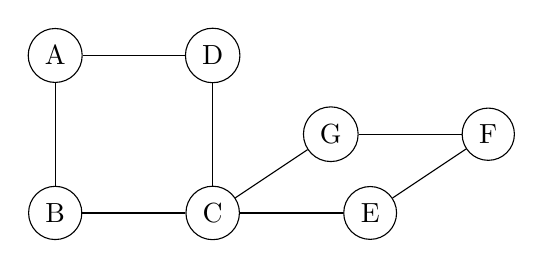
\begin{tikzpicture}
\tikzstyle{vertex} = [circle, draw=black]
\tikzstyle{edge} = [draw=black]

\node[vertex] (A) at (-1,0) {A};
\node[vertex] (B) at (-1,-2) {B};
\node[vertex] (C) at (1,-2) {C};
\node[vertex] (D) at (1,0) {D};
\node[vertex] (E) at (3,-2) {E};
\node[vertex] (F) at (4.5,-1) {F};
\node[vertex] (G) at (2.5, -1) {G};

\draw[edge] (B) -- (A);
\draw[edge] (B) -- (C);
\draw[edge] (A) -- (D);
\draw[edge] (C) -- (E);
\draw[edge] (C) -- (D);
\draw[edge] (E) -- (F);
\draw[edge] (C) -- (G);
\draw[edge] (G) -- (F);
\end{tikzpicture}
\label{fig:graf}
\end{figure}


\subsection{Begreper}

\subsubsection{Hamiltonsk sti}
En hamiltonsk sti er en sti som besøker alle nodene én gang. Dette kan virke som en triviell sak, men i en del tilfeller er det faktisk ikke mulig å finne en hamiltonsk sti. I grafen i figur \ref{fig:graf} er B, A, D, C, G, F, E en hamiltonsk sti (det finnes fler). \index{hamiltonsk sti} \index{graf!hamiltonsk sti}

Et berømt eksempel på en graf \emph{uten} en hamiltonsk sti er broene i Königsberg: \index{broene i Königsberg}
\begin{figure}[H]
\centering
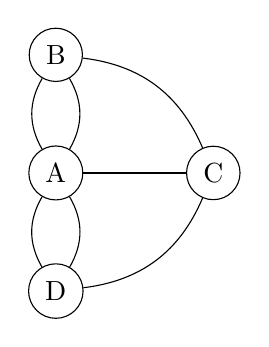
\begin{tikzpicture}
\tikzstyle{vertex} = [circle, draw=black]
\tikzstyle{edge} = [draw=black]

\node[vertex] (A) at (0,0) {A};
\node[vertex] (B) at (0,1.5) {B};
\node[vertex] (C) at (2,0) {C};
\node[vertex] (D) at (0, -1.5) {D};

\draw[edge] (A) to (C);
\draw[edge] (B) to [bend left] (C);
\draw[edge] (A) to [bend left] (B);
\draw[edge] (A) to [bend right] (B);
\draw[edge] (A) to [bend left] (D);
\draw[edge] (A) to [bend right] (D);
\draw[edge] (D) to [bend right] (C);
\end{tikzpicture}
\end{figure}



\subsubsection{Spenntrær}
Vi begynner med en definisjon:\index{spenntre} \index{minimalt spenntre}

\begin{definisjon}
Et \textbf{spenntre} for en urettet graf $ G $ er et tre med kanter fra grafen slik at alle nodene i $ G $ er forbundet. Spesielt er et \textbf{minimalt spenntre} de(t) spenntre(ene) med lavest total kostnad.
\end{definisjon}

\noindent Minimale spenntrær er sjeldent entydig bestemt. Vi har et entydig minimalt spenntre hvis alle kantene har forskjellig vekt. Vi tegner opp et eksempel:

\begin{figure}[H]
\centering
\caption{En graf (venstre) og et minimalt spenntre for grafen (høyre)}~\\
\label{fig:min_spenntre}
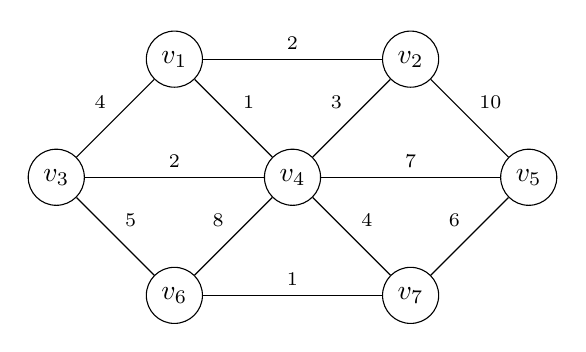
\begin{tikzpicture}[auto,node distance=2cm]
\tikzstyle{vertex} = [circle, draw=black]
\tikzstyle{edge} = [draw=black]

\node[vertex] (v1) at (-1.5,1.5) {$ v_1 $};
\node[vertex] (v2) at (1.5, 1.5) {$ v_2 $};
\node[vertex] (v3) at (-3,0) {$ v_3 $};
\node[vertex] (v4) at (0,0) {$ v_4 $};
\node[vertex] (v5) at (3,0) {$ v_5 $};
\node[vertex] (v6) at (-1.5,-1.5) {$ v_6 $};
\node[vertex] (v7) at (1.5,-1.5) {$ v_7 $};

\draw[edge] (v3) to node{\scriptsize4} (v1);
\draw[edge] (v3) to node{\scriptsize2} (v4);
\draw[edge] (v3) to node{\scriptsize5} (v6);
\draw[edge] (v1) to node{\scriptsize1} (v4);
\draw[edge] (v6) to node{\scriptsize8} (v4);
\draw[edge] (v4) to node{\scriptsize3} (v2);
\draw[edge] (v4) to node{\scriptsize4} (v7);
\draw[edge] (v4) to node{\scriptsize7} (v5);
\draw[edge] (v2) to node{\scriptsize10} (v5);
\draw[edge] (v7) to node{\scriptsize6} (v5);
\draw[edge] (v1) to node{\scriptsize2} (v2);
\draw[edge] (v6) to node{\scriptsize1} (v7);
\end{tikzpicture}~~
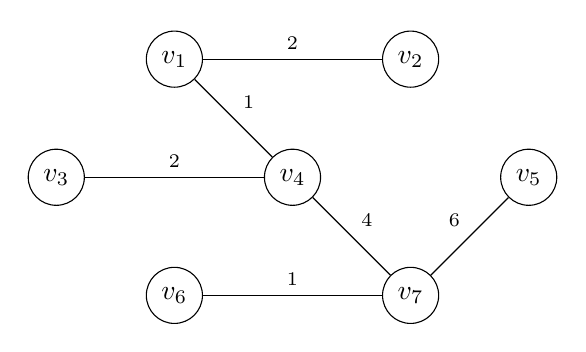
\begin{tikzpicture}[auto,node distance=2cm]
\tikzstyle{vertex} = [circle, draw=black]
\tikzstyle{edge} = [draw=black]

\node[vertex] (v1) at (-1.5,1.5) {$ v_1 $};
\node[vertex] (v2) at (1.5, 1.5) {$ v_2 $};
\node[vertex] (v3) at (-3,0) {$ v_3 $};
\node[vertex] (v4) at (0,0) {$ v_4 $};
\node[vertex] (v5) at (3,0) {$ v_5 $};
\node[vertex] (v6) at (-1.5,-1.5) {$ v_6 $};
\node[vertex] (v7) at (1.5,-1.5) {$ v_7 $};

\draw[edge] (v3) to node{\scriptsize2} (v4);
\draw[edge] (v1) to node{\scriptsize1} (v4);
\draw[edge] (v4) to node{\scriptsize4} (v7);
\draw[edge] (v7) to node{\scriptsize6} (v5);
\draw[edge] (v1) to node{\scriptsize2} (v2);
\draw[edge] (v6) to node{\scriptsize1} (v7);
\end{tikzpicture}~\\~\\
\end{figure}

For å finne et minimalt spenntre til en graf kan vi bruke Prims algoritme (\ref{prim}) eller Kruskals algoritme (\ref{kruskal})


\subsubsection{Topologisk sortering}
Topologisk sortering er en ordning av noder i en DAG slik at dersom det finnes en vei fra $ v_i $ til $ v_j $ i grafen kommer $ v_i $ før $ v_j $ i sorteringa. En topologisk sortering er ikke nødvendigvis entydig bestemt, ofte finnes det veldig mange. Hvis en graf er syklisk eksisterer det ikke en topologisk sortering av grafen. Vi ser på et eksempel: \index{topologisk sortering}

\begin{eks} Gitt følgende graf, finn alle topologiske sorteringer.
\begin{figure}[H]
\centering
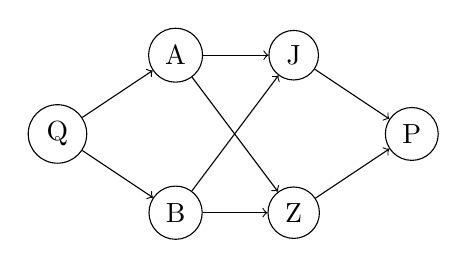
\begin{tikzpicture}[->]
\tikzstyle{v} = [circle, draw=black]
\tikzstyle{e} = [draw=black]

\node[v] (Q) at (-3, 0) {Q};
\node[v] (A) at (-1.5, 1) {A};
\node[v] (B) at (-1.5, -1) {B};
\node[v] (J) at (0, 1) {J};
\node[v] (Z) at (0, -1) {Z};
\node[v] (P) at (1.5, 0) {P};

\draw[e] (Q) to (A);
\draw[e] (Q) to (B);
\draw[e] (A) to (J);
\draw[e] (B) to (Z);
\draw[e] (B) to (J);
\draw[e] (A) to (Z);
\draw[e] (J) to (P);
\draw[e] (Z) to (P);
\end{tikzpicture}
\end{figure}

Vi ser at Q har inngrad 0, det er derfor et logisk sted å begynne. Etter Q kommer A og B. Vi ser at vi kan ikke gå videre fra A før uten å ha vært innom B, siden både J og Z er avhengige av B. Tilsvarende kan vi ikke gå videre fra B før vi har vært innom A. Til slutt ser vi at P er avhengig av både J og Z. Begge de to må derfor komme før P i sorteringa. Vi har da dekt alle mulige utfall. Vi kan liste opp alle mulige sorteringer:
\begin{itemize}
\item Q, A, B, J, Z, P
\item Q, B, A, J, Z, P
\item Q, A, B, Z, J, P
\item Q, B, A, Z, J, P
\end{itemize}

Vi kan ta med et moteksempel også: Q, A, J, B, Z, P er ikke en gyldig topologisk sortering siden J kommer før B i sorteringa, men i grafen ser vi at J er avhengig av B (det går en kant fra B til J).
\end{eks}



\subsubsection{Strongly connected components (SCC)}
Vi ser på definisjonen av strongly connected components (heretter SCC): \index{SCC (strongly connected components)}
\begin{definisjon}
Anta at vi har en rettet graf $ G = (V, E) $. Vi har da at en \textbf{SCC} av $ G $ er et maksimalt sett av noder $ U \subseteq V $ slik at for alle $ u_i $, $ u_j \in U $ har vi at $ u_i \leadsto u_j $ og $ u_j \leadsto u_i $.
\end{definisjon}

Med andre ord: en SCC er en del (partisjon) av grafen der alle nodene i den partisjonen kan nå alle andre noder i partisjonen. Vi ser på et eksempel: \index{graf!partisjon}

\begin{eks} Finn alle SCCer i grafen:
\begin{figure}[H]
\centering
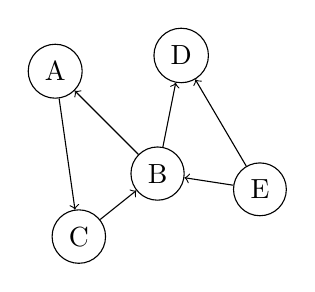
\begin{tikzpicture}[->]
\tikzstyle{v} = [circle, draw=black]
\tikzstyle{e} = [draw=black]

\node[v] (A) at (-1.3, 1.3) {A};
\node[v] (B) at (0, 0) {B};
\node[v] (C) at (-1, -.8) {C};
\node[v] (D) at (0.3, 1.5) {D};
\node[v] (E) at (1.3, -0.2) {E};

\draw[e] (A) to (C);
\draw[e] (C) to (B);
\draw[e] (B) to (A);
\draw[e] (B) to (D);
\draw[e] (E) to (B);
\draw[e] (E) to (D);
\end{tikzpicture}
\end{figure}
Vi ser at \{A, B, C\} danner en SCC. D har ingen kanter ut. Den må derfor være sin egen SCC. E ingen kanter inn, den må også være sin egen SCC. Vi har da at vi kan partisjonere grafen slik: \{\{A, B, C\}, \{D\}, \{E\} \}
\end{eks}

\subsubsection{Articulation points og biconnectivity}
Et \textbf{articulation point} er et kritisk punkt i en sammenhengende graf som ikke kan fjernes uten at grafen ikke lenger er sammenhengende. I grafen i figur \ref{fig:graf} er C et slikt punkt. Vi ser at vi kan ta vekk A uten noen store komplikasjoner, men hvis vi tar vekk C vil ikke lenger B og E være sammenknyttet.\index{graf!articulation points}

En \textbf{biconnected} graf er en graf uten articulation points, altså en graf der det alltid finnes mer enn én vei fra en node til en annen. Grafen (til venstre) i figur \ref{fig:min_spenntre} er en slik graf. \index{graf!biconnected}

\subsection{Grafalgoritmer}

\subsubsection{Dybde først}
\label{dfs}
Dybde-først-traversering (herfra dfs: depth first search) er en måte å traversere gjennom en graf på. Det kan tenkes på som en generalisering av dybde-først-traversering gjennom trær. Vi velger oss en (hvilken som helst) startnode, og beveger oss ned til etterfølgerne til noden. Når vi kommer til en node som ikke har kanter til en ubesøkt node (enten at noden har utgrad 0, eller at alle etterfølgerne er besøkt) går vi tilbake. 

Underveis i traverseringen har vi en teller som holder styr på hvor mange skritt vi har tatt. I hver node lagrer vi verdien av telleren prefix og postfix, det vil si første gang vi kommer til noden og når vi kommer tilbake etter å ha vært nedom barna. 

\begin{figure}[H]
\centering
\captionsetup{justification=centering,margin=1cm}
\caption{En rettet graf med tallene lagret etter et dfs. Heltrukne linjer er kanter vi besøkte i dfs-et, striplede linjer er kanter vi ikke besøkte}~\\
\label{fig:dfs}
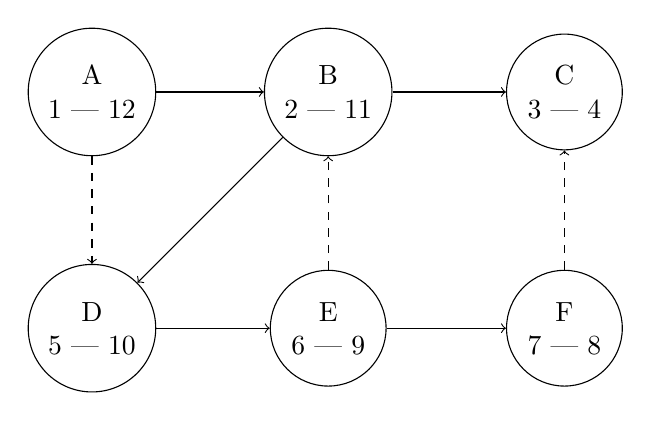
\begin{tikzpicture}[->, align=center]
\tikzstyle{v} = [circle, draw=black]
\tikzstyle{e} = [draw=black]
\tikzstyle{eh} = [draw=black, dashed]

\node[v](A) at (0, 3) {A\\1 | 12};
\node[v](B) at (3, 3) {B\\2 | 11};
\node[v](C) at (6, 3) {C\\3 | 4};
\node[v](D) at (0, 0) {D\\5 | 10};
\node[v](E) at (3, 0) {E\\6 | 9};
\node[v](F) at (6, 0) {F\\7 | 8};

\draw[e] (A) to (B);
\draw[e] (B) to (D);
\draw[eh] (A) to (D);
\draw[e] (D) to (E);
\draw[e] (E) to (F);
\draw[eh] (F) to (C);
\draw[e] (B) to (C);
\draw[eh] (E) to (B);
\end{tikzpicture}
\end{figure}

I figur \ref{fig:dfs} har vi brukt A som rotnode. Vi gikk deretter til et av barna, B. Videre gikk vi til C, og siden C har utgrad 0 måtte vi gå tilbake til B igjen. Fra B gikk vi videre til D, så til E og til F. Fra F går det en kant til C, men siden vi har besøkt C fra før går vi tilbake igjen. 

DFS-algorigmer er velegnet for å programmere rekursivt. Et eksempel på en enkel implementasjon i Java (som en metode i en Node-klasse):

\javaimport{kode/dfs.java}
\newpage

\subsubsection{Kosarajus algoritme (Finne SCC)}
Vi kan finne SCCer i en graf $ G $ ved å utføre to dfs. Et på $ G $ og et på $ G^t $, som er grafen vi får ved å snu alle kantene i $ G $. Denne algoritmen kalles Kosarajus algoritme.

\begin{teorem} Kosarajus algoritme

La $ G $ være en rettet graf. Utfør et dfs på $ G $ fra en hvilken som helst startnode, og lagre postfix-telleren (det som ble kalt \verb|highNum| i kodeekempelet i \ref{dfs}). Hvis søket slutter før alle nodene er besøkt, starter vi fra en ny, ubesøkt node.

Snu alle kantene i (transponer) $ G $ og dann $ G^t $. Sorter nodene i $ G $ synkende etter verdien på postfix-telleren. Start et dfs i $ G^t $ fra den noden som har høyest verdi. Alle nodene vi da besøker danner en SCC. Fjern så alle nodene vi besøkte fra grafen $ G^t $, og utfør et nytt dfs fra den noden som nå har høyest tellerverdi. Fortsett slik til alle nodene er besøkt. 
\end{teorem}


\noindent Vi ser på et eksempel:

\begin{eks} Finn alle SCCer i grafen:

\begin{figure}[H]
\centering
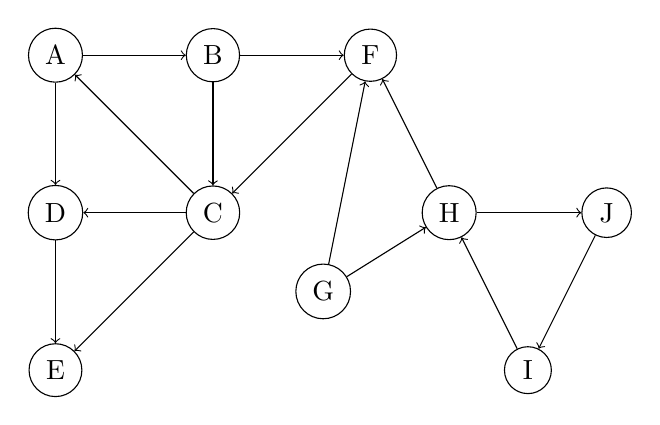
\begin{tikzpicture}[->, align=center]
\tikzstyle{v} = [circle, draw=black]
\tikzstyle{e} = [draw=black]

\node[v] (A) at (-2, 2) {A};
\node[v] (B) at (0, 2) {B};
\node[v] (C) at (0, 0) {C};
\node[v] (D) at (-2, 0) {D};
\node[v] (E) at (-2, -2) {E};
\node[v] (F) at (2, 2) {F};
\node[v] (G) at (1.4, -1) {G};
\node[v] (H) at (3, 0) {H};
\node[v] (I) at (4, -2) {I};
\node[v] (J) at (5, 0) {J};

\draw[e] (A) to (B);
\draw[e] (A) to (D);
\draw[e] (B) to (C);
\draw[e] (B) to (F);
\draw[e] (C) to (A);
\draw[e] (C) to (D);
\draw[e] (C) to (E);
\draw[e] (D) to (E);
\draw[e] (F) to (C);
\draw[e] (G) to (F);
\draw[e] (G) to (H);
\draw[e] (H) to (F);
\draw[e] (H) to (J);
\draw[e] (I) to (H);
\draw[e] (J) to (I);
\end{tikzpicture}
\end{figure}

Vi begynner med å gjøre et dfs. Vi starter i A. Søket stopper etter å ha besøkt A, B, C, D, E og F, og må starte på nytt i G. Startpunktene er valg tilfeldig, og kunne like gjerne vært noen andre. 

\begin{figure}[H]
\centering
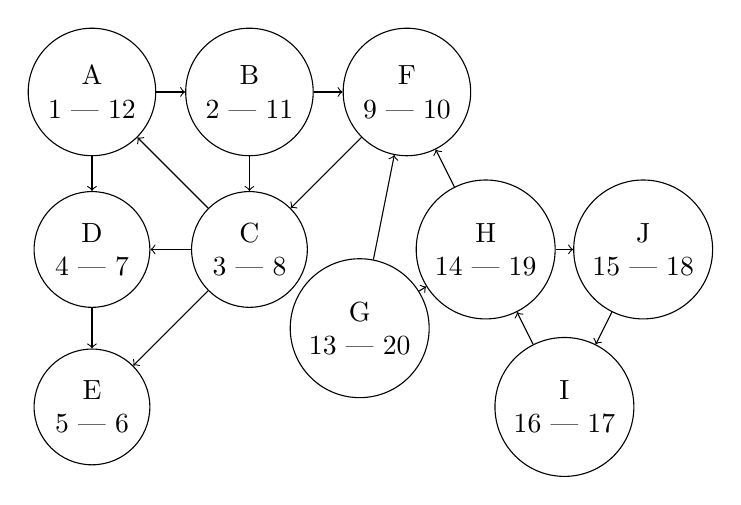
\begin{tikzpicture}[->, align=center]
\tikzstyle{v} = [circle, draw=black]
\tikzstyle{e} = [draw=black]

\node[v] (A) at (-2, 2) {A\\1 | 12};
\node[v] (B) at (0, 2) {B\\2 | 11};
\node[v] (C) at (0, 0) {C\\3 | 8};
\node[v] (D) at (-2, 0) {D\\4 | 7};
\node[v] (E) at (-2, -2) {E\\5 | 6};
\node[v] (F) at (2, 2) {F\\9 | 10};
\node[v] (G) at (1.4, -1) {G\\13 | 20};
\node[v] (H) at (3, 0) {H\\14 | 19};
\node[v] (I) at (4, -2) {I\\16 | 17};
\node[v] (J) at (5, 0) {J\\15 | 18};

\draw[e] (A) to (B);
\draw[e] (A) to (D);
\draw[e] (B) to (C);
\draw[e] (B) to (F);
\draw[e] (C) to (A);
\draw[e] (C) to (D);
\draw[e] (C) to (E);
\draw[e] (D) to (E);
\draw[e] (F) to (C);
\draw[e] (G) to (F);
\draw[e] (G) to (H);
\draw[e] (H) to (F);
\draw[e] (H) to (J);
\draw[e] (I) to (H);
\draw[e] (J) to (I);
\end{tikzpicture}
\end{figure}

\noindent Det hadde vært nok å bare lagre postfixverdiene, men vi har tatt med begge for oversiktens skyld. Vi transponerer $ G $:

\begin{figure}[H]
\centering
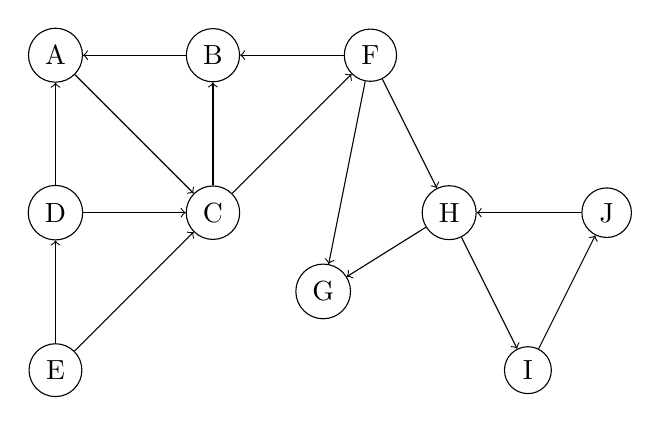
\begin{tikzpicture}[->, align=center]
\tikzstyle{v} = [circle, draw=black]
\tikzstyle{e} = [draw=black]

\node[v] (A) at (-2, 2) {A};
\node[v] (B) at (0, 2) {B};
\node[v] (C) at (0, 0) {C};
\node[v] (D) at (-2, 0) {D};
\node[v] (E) at (-2, -2) {E};
\node[v] (F) at (2, 2) {F};
\node[v] (G) at (1.4, -1) {G};
\node[v] (H) at (3, 0) {H};
\node[v] (I) at (4, -2) {I};
\node[v] (J) at (5, 0) {J};

\draw[e] (B) to (A);
\draw[e] (D) to (A);
\draw[e] (C) to (B);
\draw[e] (F) to (B);
\draw[e] (A) to (C);
\draw[e] (D) to (C);
\draw[e] (E) to (C);
\draw[e] (E) to (D);
\draw[e] (C) to (F);
\draw[e] (F) to (G);
\draw[e] (H) to (G);
\draw[e] (F) to (H);
\draw[e] (J) to (H);
\draw[e] (H) to (I);
\draw[e] (I) to (J);
\end{tikzpicture}
\end{figure}

Siden G har høyest postfixteller (20) begynner vi der. Vi ser i $ G^t $ at G ikke har noen kanter ut. Første SCC er derfor \{G\}. Når vi tar vekk G fra grafen er det H som har høyest postfixverdi (19), vi starter derfor neste dfs derfra. Vi går fra H til I og J, før vi treffer på H igjen. Vi går tilbake, men siden hverken J eller I har flere etterfølgere stopper søket, og neste SCC er derfor \{H, I, J\}. Nå er det A som har høyest postfixteller (12), så vi starter derfra. Fra A går vi til C, og til B. Da møter vi på A igjen, så vi går tilbake til C og videre til F. Vi går \emph{ikke} fra F til G eller H, siden de allerede er besøkt tidligere. Vi går derfor tilbake til C og tilbake til A. I det søke besøkte vi \{A, B, C, F\}, det blir derfor neste SCC. Til slutt starter vi i D (7), men siden D ikke har noen kanter til ubesøkte noder stopper søket med en gang. Det samme skjer i E (6). 

Alle SCCer til $ G $ er: \{ \{G\}, \{H, I, J\}, \{A, B, C, F\}, \{D\}, \{E\} \}
\end{eks}

\subsubsection{Dijkstras algoritme}
\label{dijkstra}

Dijkstras algoritme er en algoritme for å finne korteste vei fra en node til alle andre noder i en urettet graf. Algoritmen er i utgangspunktet for vektede grafer, men kan også anvendes på uvektede. Vi tenker da på en uvektet graf som en vektet graf der alle vektene er like ($ =1 $). Algoritmen er grådig siden vi alltid velger den noden med lavest avstand, og fortsetter derfra. 

\begin{teorem}Dijkstras algoritme

Vi skal finne korteste vei fra en node $ s $ til alle andre noder i en vektet, urettet graf $ G $. 
\begin{enumerate}
\item For alle noder: Sett avstanden fra startnoden $ s $ lik $ \infty $. Sett avstanden fra $ s $ til seg selv lik 0
\item Velg den naboen $ v $ til $ s $ med lavest avstand og marker den som kjent.
\item For hver nabonode $ w $ til $ v $: Dersom avstanden vi får ved å følge veien gjennom $ v $ er kortere enn den gamle avstanden, reduserer vi avstanden fra $ s $ til $ w $, og setter bakoverpekeren i $ w $ til $ v $. 
\end{enumerate}
\end{teorem}

\newpage
\noindent Vi ser på et eksempel:

\begin{eks} Finn korteste vei fra $ v1 $ til alle andre noder:
\begin{figure}[H]
\centering
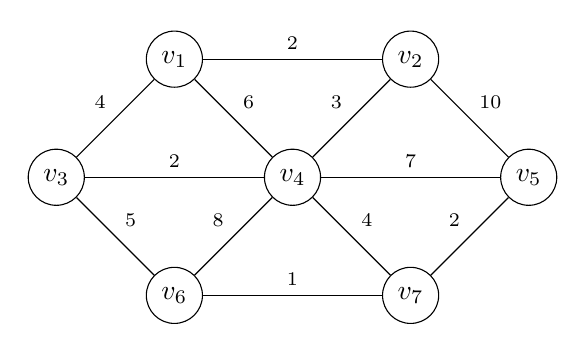
\begin{tikzpicture}[auto,node distance=2cm]
\tikzstyle{vertex} = [circle, draw=black]
\tikzstyle{edge} = [draw=black]

\node[vertex] (v1) at (-1.5,1.5) {$ v_1 $};
\node[vertex] (v2) at (1.5, 1.5) {$ v_2 $};
\node[vertex] (v3) at (-3,0) {$ v_3 $};
\node[vertex] (v4) at (0,0) {$ v_4 $};
\node[vertex] (v5) at (3,0) {$ v_5 $};
\node[vertex] (v6) at (-1.5,-1.5) {$ v_6 $};
\node[vertex] (v7) at (1.5,-1.5) {$ v_7 $};

\draw[edge] (v3) to node{\scriptsize4} (v1);
\draw[edge] (v3) to node{\scriptsize2} (v4);
\draw[edge] (v3) to node{\scriptsize5} (v6);
\draw[edge] (v1) to node{\scriptsize6} (v4);
\draw[edge] (v6) to node{\scriptsize8} (v4);
\draw[edge] (v4) to node{\scriptsize3} (v2);
\draw[edge] (v4) to node{\scriptsize4} (v7);
\draw[edge] (v4) to node{\scriptsize7} (v5);
\draw[edge] (v2) to node{\scriptsize10} (v5);
\draw[edge] (v7) to node{\scriptsize2} (v5);
\draw[edge] (v1) to node{\scriptsize2} (v2);
\draw[edge] (v6) to node{\scriptsize1} (v7);
\end{tikzpicture}
\end{figure}

\noindent Vi begynner med å sette opp en tabell over nodene:
\begin{center}
\begin{tabular}{c | c | c | l}
	 Node   & Kjent & Avstand    & Vei \\ \hline
	$ v_1 $ & T     & 0          & -   \\
	$ v_2 $ & F     & $ \infty $ & -   \\
	$ v_3 $ & F     & $ \infty $ & -   \\
	$ v_4 $ & F     & $ \infty $ & -   \\
	$ v_5 $ & F     & $ \infty $ & -   \\
	$ v_6 $ & F     & $ \infty $ & -   \\
	$ v_7 $ & F     & $ \infty $ & -
\end{tabular}
\end{center}
Vi ser på kantene ut fra $ v_1 $. Vi oppdaterer veien til $ v_2 $, $ v_3 $ og $ v_4 $:
\begin{center}
\begin{tabular}{c | c | c | l}
	 Node   & Kjent & Avstand    & Vei                    \\ \hline
	$ v_1 $ & T     & 0          & -                      \\
	$ v_2 $ & F     & $ 2 $      & $ v_1 \leftarrow v_2 $ \\
	$ v_3 $ & F     & $ 4 $      & $ v_1 \leftarrow v_3 $ \\
	$ v_4 $ & F     & $ 6 $      & $ v_1 \leftarrow v_4 $ \\
	$ v_5 $ & F     & $ \infty $ & -                      \\
	$ v_6 $ & F     & $ \infty $ & -                      \\
	$ v_7 $ & F     & $ \infty $ & -
\end{tabular}
\end{center}
Nå kommer Dijkstras grådige kriterium: Vi velger den noden som har lavest avstand til $ v_1 $ og som ikke er kjent, altså $ v_2 $ og fortsetter derfra. Fra $ v_2 $ har vi kant til $ v_4 $ og $ v_5 $. Ved å gå via $ v_2 $ får vi litt kortere avstand mellom $ v_4 $ og $ v_1 $. Vi oppdaterer tabellen:
\begin{center}
\begin{tabular}{c | c | c | l}
	 Node   & Kjent & Avstand    & Vei                                   \\ \hline
	$ v_1 $ & T     & 0          & -                                     \\
	$ v_2 $ & T     & $ 2 $      & $ v_1 \leftarrow v_2 $                \\
	$ v_3 $ & F     & $ 4 $      & $ v_1 \leftarrow v_3 $                \\
	$ v_4 $ & F     & $ 5 $      & $ v_1 \leftarrow v_2 \leftarrow v_4 $ \\
	$ v_5 $ & F     & $ 12 $     & $ v_1 \leftarrow v_2 \leftarrow v_5 $ \\
	$ v_6 $ & F     & $ \infty $ & -                                     \\
	$ v_7 $ & F     & $ \infty $ & -
\end{tabular}
\end{center}
Neste ukjente node med lavest avstand er $ v_3 $. Vi fortsetter derfra. De neste stegene ser slik ut:
\begin{center}
\begin{tabular}{c | c | c | l}
	 Node   & Kjent & Avstand    & Vei                                   \\ \hline
	$ v_1 $ & T     & 0          & -                                     \\
	$ v_2 $ & T     & $ 2 $      & $ v_1 \leftarrow v_2 $                \\
	$ v_3 $ & T     & $ 4 $      & $ v_1 \leftarrow v_3 $                \\
	$ v_4 $ & F     & $ 5 $      & $ v_1 \leftarrow v_2 \leftarrow v_4 $ \\
	$ v_5 $ & F     & $ 12 $     & $ v_1 \leftarrow v_2 \leftarrow v_5 $ \\
	$ v_6 $ & F     & $ 9 $      & $ v_1 \leftarrow v_3 \leftarrow v_6 $ \\
	$ v_7 $ & F     & $ \infty $ & -
\end{tabular}~~
\begin{tabular}{c | c | c | l}
	 Node   & Kjent & Avstand & Vei                                                  \\ \hline
	$ v_1 $ & T     & 0       & -                                                    \\
	$ v_2 $ & T     & $ 2 $   & $ v_1 \leftarrow v_2 $                               \\
	$ v_3 $ & T     & $ 4 $   & $ v_1 \leftarrow v_3 $                               \\
	$ v_4 $ & T     & $ 5 $   & $ v_1 \leftarrow v_2 \leftarrow v_4 $                \\
	$ v_5 $ & F     & $ 12 $  & $ v_1 \leftarrow v_2 \leftarrow v_5 $                \\
	$ v_6 $ & F     & $ 9 $   & $ v_1 \leftarrow v_3 \leftarrow v_6 $                \\
	$ v_7 $ & F     & $ 9 $   & $ v_1 \leftarrow v_2 \leftarrow v_4 \leftarrow v_7 $
\end{tabular}
\end{center}

\begin{center}
\begin{tabular}{c | c | c | l}
	 Node   & Kjent & Avstand & Vei                                                  \\ \hline
	$ v_1 $ & T     & 0       & -                                                    \\
	$ v_2 $ & T     & $ 2 $   & $ v_1 \leftarrow v_2 $                               \\
	$ v_3 $ & T     & $ 4 $   & $ v_1 \leftarrow v_3 $                               \\
	$ v_4 $ & T     & $ 5 $   & $ v_1 \leftarrow v_2 \leftarrow v_4 $                \\
	$ v_5 $ & F     & $ 12 $  & $ v_1 \leftarrow v_2 \leftarrow v_5 $                \\
	$ v_6 $ & T     & $ 9 $   & $ v_1 \leftarrow v_3 \leftarrow v_6 $                \\
	$ v_7 $ & F     & $ 9 $   & $ v_1 \leftarrow v_2 \leftarrow v_4 \leftarrow v_7 $
\end{tabular}
\end{center}
\begin{center}
\begin{tabular}{c | c | c | l}
	 Node   & Kjent & Avstand & Vei                                                                 \\ \hline
	$ v_1 $ & T     & 0       & -                                                                   \\
	$ v_2 $ & T     & $ 2 $   & $ v_1 \leftarrow v_2 $                                              \\
	$ v_3 $ & T     & $ 4 $   & $ v_1 \leftarrow v_3 $                                              \\
	$ v_4 $ & T     & $ 5 $   & $ v_1 \leftarrow v_2 \leftarrow v_4 $                               \\
	$ v_5 $ & F     & $ 11 $  & $ v_1 \leftarrow v_2 \leftarrow v_4 \leftarrow v_7 \leftarrow v_5 $ \\
	$ v_6 $ & T     & $ 9 $   & $ v_1 \leftarrow v_3 \leftarrow v_6 $                               \\
	$ v_7 $ & T     & $ 9 $   & $ v_1 \leftarrow v_2 \leftarrow v_4 \leftarrow v_7 $
\end{tabular}
\end{center}
\begin{center}
\begin{tabular}{c | c | c | l}
	 Node   & Kjent & Avstand & Vei                                                                 \\ \hline
	$ v_1 $ & T     & 0       & -                                                                   \\
	$ v_2 $ & T     & $ 2 $   & $ v_1 \leftarrow v_2 $                                              \\
	$ v_3 $ & T     & $ 4 $   & $ v_1 \leftarrow v_3 $                                              \\
	$ v_4 $ & T     & $ 5 $   & $ v_1 \leftarrow v_2 \leftarrow v_4 $                               \\
	$ v_5 $ & T     & $ 11 $  & $ v_1 \leftarrow v_2 \leftarrow v_4 \leftarrow v_7 \leftarrow v_5 $ \\
	$ v_6 $ & T     & $ 9 $   & $ v_1 \leftarrow v_3 \leftarrow v_6 $                               \\
	$ v_7 $ & T     & $ 9 $   & $ v_1 \leftarrow v_2 \leftarrow v_4 \leftarrow v_7 $
\end{tabular}
\end{center}
\end{eks}

\paragraph{Tidsanalyse}~\\
Hvis vi søker gjennom grafen etter den noden med lavest avstand vil det ta $ O(|V|) $ tid, og dette gjør vi $ |V| $ ganger. Total tid for å finne minste avstand er derfor $ O(|V|^2) $. I tillegg må vi oppdatere avstandene. Det er maksimalt én oppdatering for hver kant, det vil si at det tilsammen tar $ O(|E|) $. Total kjøretid for algoritmen er derfor:
\[ \text{Kjøretid} = O\left(|V|^2 + |E|\right) = O\left(|V|^2\right) \]

\subsubsection{Prims algoritme}
\label{prim}

Prims algoritme er en algoritme for å finne minimale spenntrær. Det er en grådig algoritme siden den bygger treet trinnvis ved å velge den kanten som går ut av treet med lavest vekt. 

\begin{teorem} Prims algoritme

Vi skal finne et minimalt spenntre for en graf $ G $. Velg først en startnode (rotnode). Den kan velges helt tilfeldig. Så lenge treet ikke spenner hele $ G $ legger vi til den kanten fra treet, til en ukjent node som har lavest vekt.
\end{teorem}

\noindent Vi ser på et eksempel.

\begin{eks} Finn et minimalt spenntre for grafen i figur \ref{fig:min_spenntre}.

Vi velger $ v_1 $ som rotnode (vi kunne valgt hvilken som helst annen). Den kanten med lavest vekt ut fra treet (som kun består av $ v_1 $) er kanten $ v_1-v_4 $, så vi legger den til. Videre er kanten $ v_1-v_2 $ den kanten med lavest vekt som går til en ukjent node, så vi legger til den. $ v_4-v_3 $ er neste kant vi legger til. Kanten $ v_2-v_4 $ er nå den kanten med lavest vekt som går ut fra treet, men siden $ v_2 $ og $ v_4 $ begge er inneholdt i treet er ikke den interessant. Neste kant vi legger til er $ v_4-v_7 $, deretter $ v_7-v_6 $ og $ v_7-v_5 $. Treet er nå et komplett spenntre for $ G $. 
\end{eks}

\paragraph{Tidsanalyse}~\\
Samme argument som tidsanalysen til Dijkstra. Total kjøretid: $ O\left(|V|^2\right) $


\subsubsection{Kruskals algoritme}
\label{kruskal}

Kruskals algoritme er en annen algoritme for å finne minimale spenntrær. Det er også en grådig algoritme, siden vi til enhver tid velger den kanten med lavest vekt som ikke danner en løkke.

\begin{teorem} Kruskals algoritme

Vi skal finne et minimalt spenntre for en graf $ G $. La $ F $ være en skog (en mengde av trær). Så lenge $ F $ ikke utspenner alle nodene velger vi den kanten med lavest vekt fra $ G $, og som ikke danner en løkke, og legger den til i $ F $. Når $ F $ har blitt ett sammenhengende tre og alle nodene er nådd har vi et minimalt spenntre.
\end{teorem}

\noindent Vi ser på et eksempel.

\begin{eks} Finn et minimalt spenntre for grafen i figur \ref{fig:min_spenntre}.

Vi finner kanten(e) i grafen med den minste vekten. $ v_6-v_7 $ og $ v_1-v_4 $ har begge vekt 1. Vi legger de til i spenntreet. Kantene $ v_3-v_4 $ og $ v_1-v_2 $ har begge vekt 2, og ingen av dem danner en løkke, så vi legger dem til i spenntreet. Neste kant med lavest vekt er $ v_2-v_4 $ (3), men den vil danne en løkke, så vi hopper over den. Videre ser vi at $ v_1-v_3 $ og $ v_4-v_7 $ begge har vekt 4. Kanten $ v_1-v_3 $ vil danne en løkke så den hopper vi over, men $ v_4-v_7 $ legger vi til. Neste kant med lavest vekt, og som ikke danner en løkke er $ v_5-v_7 $. Vi legger den til i spenntreet, og da er alle noder nådd, og vi har en sammenhengende graf. Vi har derfor et minimalt spenntre (se figur \ref{fig:min_spenntre}). 
\end{eks}


\paragraph{Tidsanalyse}~\\
Vi må loope gjennom alle kantene én gang, det gir tid $ O(|E|) $. Vi kan implementere algoritmen ved hjelp av en stack. Gjør vi det må vi utføre én sletting, to søk og en union. Sletting og søk tar $ O(\log_2 n) $ tid (for sletting er $ n = |E| $, for søk er $ n = |V| $), og union tar $ O(1) $ tid. For hver iterasjon har vi da:

\[ \text{Kjøretid, hver iterasjon} ~=~ O(\log_2 |E| + \log_2 |V| + 1) ~=~ O(\log_2 |V|) \]

\noindent Siste likhet har vi siden $ |V| > |E| $. Vi kan dermed sette opp total kjøretid:

\[ \text{Kjøretid, total} ~=~ O(|E| \cdot \log_2 |V|) \]


~\\
\paragraph{Prim vs Kruskal}~\\
Prim er som regel noe mer effektiv enn Kruskal, spesielt på tette grafer. Prim har likevel den svakheten at den kun fungerer på sammenhengende grafer. Kruskal anvendt på en usammenhengende graf vil gi et minimalt spenntre for hver sammenhengende del av grafen.


\subsubsection{Floyds algoritme}
\label{floyd}

Floyds algoritme er en algoritme som beregner korteste vei fra alle noder til alle andre noder. Algoritmen er et eksempel på en algoritme som benytter seg av dynamisk programmering. 

\begin{teorem} Floyds algoritme

Denne betraktningen gjentas systematisk for alle tripler i, k og j:
\begin{itemize}
\item Initielt: Avstanden fra node $ i $ til node $ j $ settes lik vekten på kanten fra $ i $ til $ j $, uendelig hvis det ikke går noen kant fra $ i $ til $ j $
\item Trinn 0: Se etter forbedringer ved å velge node 0 som mellomnode
\item Etter trinn $ k $: Avstanden mellom to noder er den korteste veien som bare bruker nodene $ 0, 1, ... , k $ som mellomnoder
\end{itemize}
\end{teorem}

\noindent Eksempel på implementasjon i Java:
\javaimport{kode/floyd.java}

\paragraph{Tidsanalyse}~\\
Vi ser fra kodeeksempelet at det er to løkker som må kjøres gjennom. En dobbel og en trippel for-løkke. Kjøretiden blir derfor:

\[ \text{Kjøretid} ~=~ O\left(n^2 + n^3\right)  ~=~ O\left(n^3\right) \]

~\\
\paragraph{Hvordan tolke input/output fra Floyds algoritme}~\\
Ved start inneholder \verb|nabo[i][j]| lengden av kanten fra $ i $ til $ j $, \verb|nabo[i][j] = |$ \infty $ hvis det ikke er noen kant. Algoritmen lar \verb|nabo| være uendret, og legger resultatene i \verb|avstand| og \verb|vei|. \verb|avstand[i][j]| er lengden av korteste vei fra $ i $ til $ j $. Når vi oppdager at den korteste veien fra $ i $ til $ j $ går gjennom $ k $ setter vi \verb|vei[i][j] = k|. \verb|vei| sier derfor om den korteste veien. Vi finner korteste vei slik:
\begin{itemize}
\item \verb|k1 = vei[i][j]| er den største verdien av $ k $ slik at $ k $ ligger på den korteste veien fra $ i $ til $ j $
\item \verb|k2 = vei[i][k1]| er den største verdien av $ k $ slik at $ k $ ligger på den korteste veien fra $ i $ til $ k_1 $
\\ $ \vdots $
\item Når \verb|vei[i][km] = -1| er $ (i, k_m) $ den første kanten i korteste vei fra $ i $ til $ j $
\end{itemize}
Dermed er korteste vei fra $ i $ til $ j $ slik: $ i \rightarrow k_m \rightarrow k_{m-1} \rightarrow ... \rightarrow k_2 \rightarrow k_1 \rightarrow j $. 